\documentclass[12pt]{article}  % for review and submission
%\documentclass[aps,preprint,showpacs,superscriptaddress,groupedaddress]{revtex4}  % for double-spaced preprint
\usepackage{graphicx}  % needed for figures
\usepackage{dcolumn}   % needed for some tables
\usepackage{bm}        % for math
\usepackage{amssymb}   % for math
\usepackage{hyperref}  %to use \autoref to reference objects
\usepackage[export]{adjustbox} %alignment of figures

%\linespread{1.8} %double-spacing

% \usepackage[hmarginratio=1:1,top=15mm, bottom=15mm, left=15mm, right=15mm,columnsep=20pt]{geometry} % Document margins
\usepackage{anysize}
\marginsize{20mm}{20mm}{20mm}{20mm}
%\marginsize{left}{right}{top}{bottom}
%\usepackage[left = 15mm, top = 15mm]{geometry} %margins

%%%%%%%%%%%%%%%%%%%%%%%%%%%%%%%%%%%%%%%%%%%%%%%%%%%%%
%%%%%%%%%%%%%%%%% COMMANDS %%%%%%%%%%%%%%%%%%%%%%%%%%
\providecommand{\e}[1]{\ensuremath{\times 10^{#1}}} %for scientific notation
\providecommand{\squiggle}{\raise.17ex\hbox{$\scriptstyle\sim$}} %for tilde character
\providecommand{\noNe}[1]{{${#1}\times 10^{19}$ cm$^{-3}$}} % for writing density as a number followed by cm^-3
\providecommand{\pow}[1]{{$^{#1}$}} % for writing a power in math mode (i.e. for units)

%%******** need tilde after variable names so there is a space between them and the following word **********
\providecommand{\neupstream}{$n_{e~upstream}~$} % upstream electron density shortcut
\providecommand{\neus}{$n_{e~us}~$} % upstream electron density shortcut
\providecommand{\netarget}{$n_{e~target}~$} % target electron density shortcut
\providecommand{\netg}{$n_{e~tg}~$} % target electron density shortcut
\providecommand{\Tus}{$T_{us}~$} % Upstream temperature shortcut
\providecommand{\Ttg}{$T_{tg}~$} % Target temperature shortcut

%\usepackage[left = 15mm, top = 15mm]{geometry} %margins
\usepackage{amssymb} % Allows use of \therefore command to get the three dots in a triangle symbol

%Figures
\usepackage{graphicx}
%syntax:
%\includegraphics[scale=1.0]{filepath.extension}

%bibliog
\usepackage[UKenglish]{babel}
\usepackage{url}
\usepackage[backend=bibtex, style=numeric-comp, sorting=none, doi=false,isbn=false,url=false]{biblatex}
\bibliography{BIBfiles/initial}
% bun citep amirite!!!
\newcommand{\citep}[1]{\cite{#1}}
%stop paper titles being printed in bibliography
\AtEveryBibitem{\clearfield{title}}
%stop "In:" being printed before journal name
\renewbibmacro{in:}{}
%small bibliography font size
\renewcommand*{\bibfont}{\small}

% Appendix
\usepackage[toc,page]{appendix}
%euro symbol (\EUR i think)
\usepackage{eurosym}

% for multirow command in table generation
\usepackage{multirow}
% make caption font small
\usepackage[font={footnotesize}]{caption}

% make things transparent (here want PRad fig a little transparent)
\usepackage{transparent}

% Document
\begin{document}

\title{Divertor detachment stability and dynamics}
\author{Joe Allen, JOA509}
%\date{\today}

%\twocolumn[
%\begin{@twocolumnfalse}
    \maketitle
    \begin{abstract}
\noindent Abstract to be written
	\end{abstract}
%\end{@twocolumnfalse}
%]

%\tableofcontents

\section{Background and Introduction}\label{secBg}
Magnetic fusion devices, specifically tokamaks, produce large amounts of power which must be contained within the machine. Current designs shape the magnetic field so as to have a divertor region, where plasma and impurities ejected from the core are funnelled and extracted. Due to the incredibly high temperatures of the ejected matter, the solid surfaces of the divertor must be protected lest they melt. Detachment promises the ability to retain the structural and functional health of the divertor while maintaining core plasma performance.

Heat fluxes entering the scrape-off layer (SOL) in current tokamaks are mitigated by several methods including neutral gas puffing and angular offsetting the divertor plates to spread the flux over a wider area. In ITER, the SOL heat flux will be far higher, around 1 GW m\pow{-2} \cite{Loarte2007}, undermining the capability of present cooling methods. This will expose the divertor plates to minimum flux of 10 MW m\pow{-2} during normal operation, with peak power fluxes during ELMs of twice that amount \cite{Loarte2007}; heat fluxes below 10 MW m\pow{-2} are required by current materials. This high power flux is unavoidable, as $ P_{SOL} \approx 100$ MW, the power entering the SOL, is fixed, and the SOL heat channel is estimated to be around 1 mm \cite{Eich2013}, and depends on factors innate to reactor design. Since these high heat fluxes entering the SOL cannot be changed, ways must be found to reduce them throughout the divertor region.

Detachment is loosely defined as when the target temperature falls below 5 eV \cite{Porter1996}, and the upstream temperature no longer dictates \Ttg. Attached plasmas are characterised by high target densities, ion current and target temperature. Detachment initiates steep drops in \Ttg, \netarget and ion current to the divertor sheath (or target plate) \cite{Stacey2001}, as well as extensive parallel pressure loss from the target toward the upstream \cite{Nakazawa2000}. Many problems arise when attempting to control the stability of detachment in experiments \cite{Lipschultz2016}, which ideally aim to fix the low temperature and pressure detached region between the X-point and target, in order to prevent it impacting on core performance. More detailed understanding of the processes behind detachment is needed in order to decide how best to control its stability in current and future tokamaks \cite{Reimold2015}. A detached divertor regime was first achieved by gas fuelling, which acted as a sink for parallel plasma momentum through charge exchange collisions \cite{Loarte1998}, combined with sufficient volumetric recombination \cite{Wischmeier2009} enough ions and momentum is removed from the SOL plasma, cooling the region close to the target and initiating detachment.

We investigate Super-X divertor (SXD) geometry, as well as conventional divertor (CD) geometry, as the extended SXD leg is thought to allow more control over the extent of detachment \cite{Valanju2009}. Divertor geometry has been shown in simulation and experiment to have large effects on the extent of detachment over a variety of operating conditions \cite{Pitts2001}. Linear plasma devices have been used to simulate divertor detachment \cite{Nishijima2002, Ohno2002}, as changes to tokamak divertors are costly both monetarily and in time.

\subsection{SOL1D}\label{ssecSOL1D}
SOL1D models a field line in the separatrix from the outboard midplane to the divertor plate, stretched out into a straight line. The section between midplane and X-point is where heat and particles enter the system from the core plasma; no heat enters between the X-point and the target, and particles only enter this region when they are recycled from the walls.

In order to study detachment, and volumetric processes along the whole length of the SOL, such as friction between plasma and neutral flows, the evolution of the properties of the divertor plasma must be known. Parallel transport in a plasma, following the direction of the magnetic field, is well understood. Therefore producing a 1-dimensional model of the SOL does not require a great deal of complexity past the 1D fluid equations. These equations are derived from integrals of successive moments of the 1D Fokker-Planck kinetic vector equation \cite{Stangeby}.

  \begin{equation}\label{eqDensity}
  \frac{\partial n}{\partial t} = -\nabla . (\textbf{b}V_{\parallel}n) + S_n - S
  \end{equation}

Plasma density is evolved as in equation~\ref{eqDensity} where $S_n$ is the external source of plasma ions and $S=R_{rec} - R_{iz}$ (recombination rate minus ionisation rate) is the net recombination of plasma particles, or a source of neutrals. The variation of plasma density at a given region depends on the rate of plasma particles leaving that point, the source of plasma particles to the area, and the net conversion of plasma to neutrals in that region.

  \begin{equation}\label{eqMomentum}
  \frac{\partial}{\partial t}(m_i n V_{\parallel}) = -\nabla . (m_i n V_{\parallel} \textbf{b} V_{\parallel}) + \partial_{\parallel}p - F
  \end{equation}

Momentum evolution, described in equation~\ref{eqMomentum}, evolves the balance between the plasma flow momentum, $m_inV_{\parallel}\textbf{b}V_{\parallel}$ where $\textbf{b}$ is the unit vector in the direction of the magnetic field, and the parallel pressure, with the addition of F as the loss of momentum of the ions due to recombination and charge exchange. The plasma flow momentum term is an average over the fluid, whereas $\partial_{\parallel}p$ is part of the inertia of the plasma.

The plasma pressure, $ p $, is evolved according to equation~\ref{eqPressure}. Here, $ E $ is the plasma energy sink to neutrals, $ R $ is the plasma energy sink by radiative losses and $ S_p $ is the external source of pressure. Plasma temperature is assumed to be uniform, $ T_i = T_e $.

  \begin{equation}\label{eqPressure}
  \frac{\partial}{\partial t}\left( \frac{3}{2}p\right)  = -\nabla.q + V_{\parallel} \partial_{\parallel}p -E - R + S_p
  \end{equation}


At the target, normal sheath boundary conditions are applied, meaning the ion velocity when entering the sheath is at least the sound speed, $ V_{\parallel}^{sheath} \geq C_s$. Particles enter the upstream at such a rate as to keep the upstream density constant, as specified in the input file. However, the particles are placed into the upstream so as not to affect parallel conservation of mass, momentum or energy ($ \partial_{\parallel}n =0, V_{\parallel} =0, \partial_{\parallel}p =0 $). Additionally, the model assumes local ambipolarity, meaning that the parallel current density, $j_{\parallel}$, throughout the 1D system is zero \cite{Stangeby}. 

Classical ion heat transport, $q_{\parallel}$, is proportional to the temperature gradient, $\nabla T$, in the SOL and is known as the Braginskii heat flux relation \citep{Braginskii1965}. This model works well at low temperatures and when the collisional mean free path is short compared to the system's scale lengths. Alternatively it assumes that particles undergo frequent collisions. However, when $\nabla T$ is very high, the scale length over which the temperature changes by a large amount (a system scale length) becomes fairly close to the size of the collisional mean free path. Consequently, the model over estimates the heat flux at high $\nabla T$ because some particles' collision lengths are very large, and hence they travel most of the SOL unhindered, meaning the model breaks down because particles do not experience frequent collisions.

The Braginskii model would produce infinitely fast heat conduction with an infinite temperature gradient. Clearly this is not possible, given that the plasma species, which are the conductors, have finite speeds. The thermal electron velocity sets the upper limit on heat transport in a real plasma, as heat cannot travel faster than the fastest particles. The free-streaming heat flux model includes this limit, and is therefore more apt to describe heat transport in a plasma model.

\subsection{Two-point model}\label{ssec2PT}
The simplest model of the divertor leg is the two-point model, which only considers differences between the upstream and target. Given that the main aim of SOL modelling is to seek ways to reduce the extremely high fluxes at the upstream before they reach the target, for simple analysis only the effect on the target of upstream variations need to be noted. This model is often used to analyse experimental data, as taking measurements between the upstream and the target can be rather difficult. It incorporates the idea of pressure balance, that the total pressure is the sum of the static and dynamic pressures:

  \begin{equation}\label{eqPbal}
  p_{tot} = p_{static} + p_{dynamic} = 2nkT + mnv^2.
  \end{equation}

Using the velocity boundary conditions of $ v_u=0 $ at the upstream and $ v_t=(2kT_t/m)^{1/2} $, the sound speed, equation~\ref{eqPus_tg} is derived. This shows the relationship between upstream and target pressure.

  \begin{equation}\label{eqPus_tg}
  n_uT_u = 2n_tT_t
  \end{equation}

\textbf{DESIRABLE ADDITIONS - Applicability of Detachment in areas other than fusion: Coronal Loops exhibiting detachment (need to flick through the 2 papers I have on this topic) 
Prominences: A. De Groof, et al, A and A 443, 319–328 (2005)}\\

\textbf{Coronal Rain: P. Antolin et al, 280 (2012) 457.}\\


We first investigate how SOL1D, a one dimensional fluid equation code, deals with detachment and confirm that factors influencing detachment in experiment and other simulations have similar effects on the state of detachment. Following this, the underlying processes causing detachment are examined in an effort to better understand this phenomenon which is likely to prove vital for future high power tokamaks. Detachment stability is very susceptible to upstream variation and other external factors, for example upstream density and impurity fraction \cite{Lipschultz2016}, and needs better understanding before detachment can be successfully controlled throughout a range of operating scenarios in ITER and other future machines. 


\section{Experimental Design}\label{secExpt}
Simulations run with SOL1D used a plasma fluid model with the partial differential equations detailed in section~\ref{secBg} (equations~\ref{eqDensity}, \ref{eqMomentum} and \ref{eqPressure}) solved iteratively over a 1D grid. Divertor neutral population is evolved according to a diffusive model, where a recycling fraction and neutral lifetime may be set depending on the desired neutral conditions. The main input parameters for these simulations are upstream density, SOL power flux input, number of grid cells, and impurity fraction. The system is initialised with uniform density and temperature, then the chosen parameter values are injected in and the density, pressure and particle flux (for both plasma and neutrals) are calculated over the grid at each time step. A steady state solution then takes varying amounts of time to materialise, depending on the extent of the differences between the initial state and the initial conditions imposed on the system, as violent sound waves travel back and forth between the upstream and target before the system starts to converge. Particle, momentum and energy sinks are also calculated, including volumetric radiative losses.

The first aim was to ascertain an acceptable grid resolution, ny, to use, as a compromise is required concerning accuracy of results and time taken to run a simulation. SOL1D performs 1-dimensional simulations and the y-axis was chosen as the simulation axis. 

\textbf{\textit{Reword}: After a number of time-steps a SOL1D simulation will usually converge and approach a steady-state solution.} This can be seen in figure~\ref{figne_var_ny=800} - the variable's, \neupstream, oscillations are damped to a very small amplitude as the simulation progresses and it approaches steady-state, which took about 24 hours to reach its current point. Perhaps the simulation could have been stopped earlier, however this would increase the uncertainty in all the output data. Simulations with lower resolution do not reach a steady state in fewer time points, but they are faster to run so they reach it quicker in real time.

\begin{figure}
	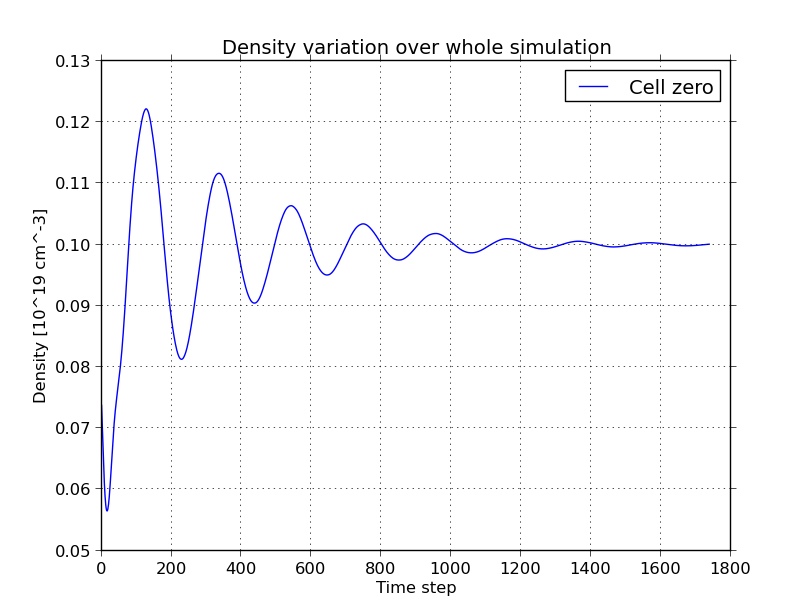
\includegraphics[scale=0.4]{Figures/sol1d/ne_var_ny=800.png}
	\centering
	\caption{The variation of \neus, [1\e{20} cm\pow{-3}], with simulation time step. }\label{figne_var_ny=800}
\end{figure}

An important first step when running grid simulations is to ascertain an acceptable resolution to use. Figure~\ref{figRE_neres1000} shows the approximate steady-state value of \netarget for different resolutions. The choice of resolution has to take into account the accuracy of the output and the time taken to receive said output. It is clear that \netg is tending towards a real value at infinite resolution, and the percentage changes between increasing resolutions are shown in table~\ref{tabsol1dres}. Given that the number of operations performed by the code scales as approximately $N^2$, for $N$ cells, increasing the cell number heavily increases the computing cost. Table~\ref{tabsol1dres} contains run times at different resolutions, and shows a stark increase in time for increasing resolution. The second run, at \neus $= 1.25\e{19}$ cm$^{-3}$, completed significantly faster than the first run because it was restarted from the near steady-state snapshot at the end of the first run. Therefore, each simulation time step is completed faster because the system is already rather stable, and only needs to accommodate an injection of an extra $0.25\e{19}$ cm$^{-3}$ of material into the upstream.

\begin{table}[]
	\centering
	\caption{SOL1D simulation run times, using 8 cores, and percentage change in \netg for different y-axis resolutions, ny.}
	\label{tabsol1dres}
	\begin{tabular}{c|c|c|c|c|c}
		\multicolumn{1}{l|}{\multirow{2}{*}{}}   & \multicolumn{2}{l|}{Time taken to complete 1000 time steps}  & \multicolumn{2}{l|}{Value and percentage change of \netg} \\ \cline{2-5} 
		Resolution          & \neus = $1.0$ & \neus = $1.25$  & \netg & \% change  \\ \hline
		200                 &      0:47:44    \qquad   &    0:24:23        &  0.2540  &   -    \\
		400                 &      1:48:55    \qquad   &    2:45:04        &  0.2674  &  5.0   \\
		600                 &      7:40:57    \qquad   &    5:05:04        &  0.2718  &  1.6   \\
		800                 &     13:18:55    \qquad   &    7:01:28        &  0.2734  &  0.6   \\
	   1000                 &  \textgreater~30h \qquad &       N/A         &  0.2745  &  0.4
	\end{tabular}
\end{table}

\begin{figure}
	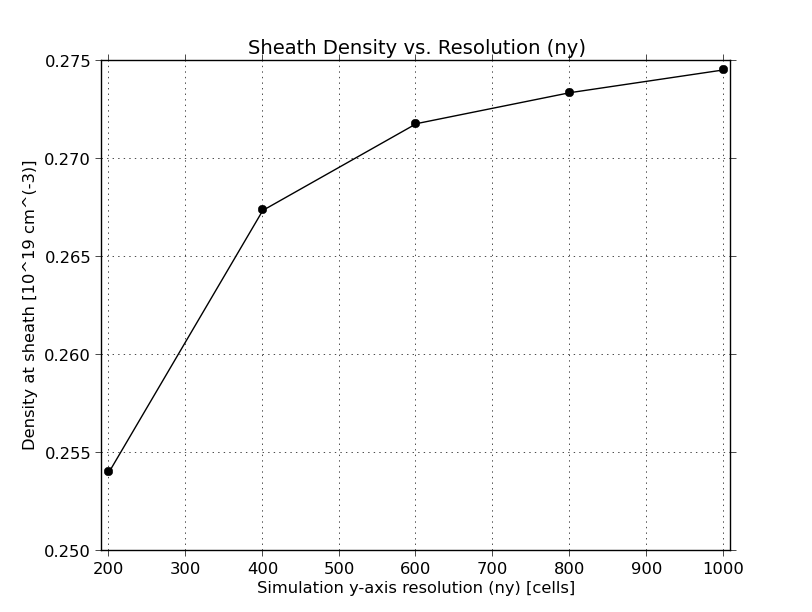
\includegraphics[scale=0.48]{Figures/sol1d/RE_neres1000.png}
	\centering
	\caption{Density at sheath, \netg, at approximately steady-state for different y-axis resolutions in SOL1D.}\label{figRE_neres1000}
\end{figure}

Detachment can be seen occurring when examining the density profiles of different simulations, figure~\ref{figneprofneusALLtriang} shows systems in varying states of detachment caused by differing set upstream densities. Although the precise point at which an attached system becomes detached can be debated. Panel a) shows an attached system, and even the higher resolution cases struggle to resolve the density profile close to the target, which is why the profiles are very jagged. Panel b) displays a detached system: the density profile peak has shifted away from the target plate somewhat, cooling the divertor surface. The density profile in panel c) is also detached from the target, but more so than in panel b), as although the profile shape adjacent to the target is a similar shape the peak has shifted toward the upstream. Once the density profile has retreated from the target it is much more easily resolved, as the peak is spread over many more cells than when it sits close to the surface. However, the low resolution case, with 200 cells along the y-axis, still struggles to produce a smooth profile close to the plate even when the system is quite detached. 

\begin{figure}
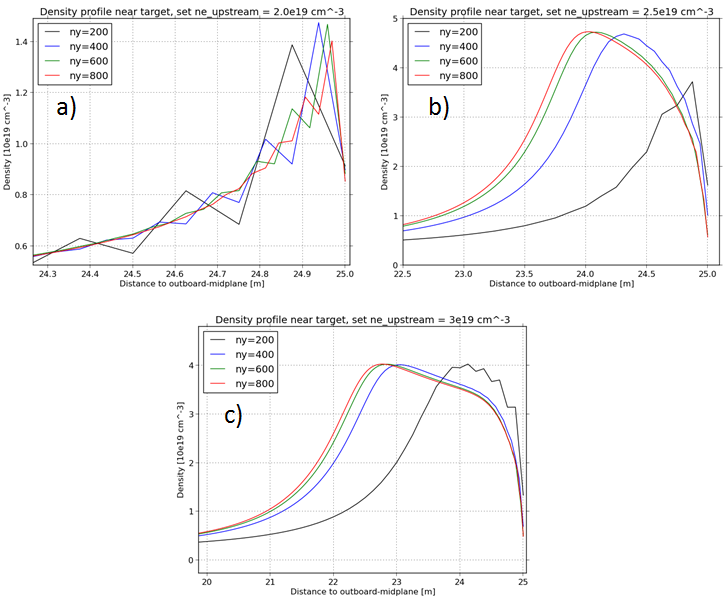
\includegraphics[scale=0.8]{Figures/sol1d/neprofneusALLtriang.png}
\centering
\caption{Density profile close to target for y-axis resolutions 200, 400, 600 \& 800 cells at different set values of \neus in SOL1D. The y-axes show the density, with units [1\e{20} cm\pow{-3}] and the x-axes show the distance to the outboard midplane in metres. Panel a) has set upstream density of \noNe{2}, panel b) was run with \neus = \noNe{2.5} and c) with \noNe{3}}\label{figneprofneusALLtriang}
\end{figure}

These density profiles in figure~\ref{figneprofneusALLtriang} provide further evidence of the necessity of using a high enough resolution in grid-based simulations. The difference between the red (800 y-axis cells) and green (600) profiles is small compared to that with blue (400) or black (200), hence a resolution of 600 cells along the y-axis seems to attain sufficiently accurate results. Unless otherwise stated, subsequent SOL1D results were taken from simulations with ny = 600 cells.

SOL1D excels as a fast 1-dimensional simulator and includes important underlying processes such as 3-body recombination, on top of expected contributions to plasma dynamics, for example impurity radiation and momentum transfer between plasma and neutrals. However, the model is missing detailed cross field transport, which is only applicable in 2-dimensional models; only an estimate for non-parallel plasma transport can be made in a 1D simulation. Furthermore, both 2 and 1D models cannot include turbulence effects, which are likely to play a role in detachment stability in real machines. Another key factor not implemented in SOL1D is impurity transport. Impurities are present as a fraction of plasma density, and evolving the impurity density profile may reduce the stability of detachment if the impurities are transported towards the upstream by interactions with the plasma \cite{Nakazawa2000}.

\section{Results and Analysis}\label{secResults}
%\subsection{SOL1D}\label{ssecSOL1D}
\subsection{Temperature comparison}\label{ssectempcomp}
Two key parameters to be analysed are the upstream and target temperatures, \Tus and \Ttg. The purpose of divertor detachment is to reduce the power flux impacting on the divertor. \Ttg sets the voltage across the sheath, which in turn influences the velocity of ions impacting on the solid divertor target (ions in the simulation have a fixed velocity when entering the sheath - the Bohm velocity). The lower \Ttg, the less damage will be done to the divertor plates. Figure~\ref{figTT_IMPCOMBO2} shows the difference between \Tus and \Ttg for different \neus values at each of the resolutions in table~\ref{tabsol1dres}. When looking to reduce \Ttg, the trade off is the corresponding fall in \Tus. As the upstream is at the SOL midplane, any changes there will be translated directly into the main plasma. 

Similarly shaped temperature profiles are observed for all resolutions in figure~\ref{figTT_IMPCOMBO2}, \Tus falls slowly while \Ttg falls rapidly with increasing \neus, until above $2.25\e{19}$ cm$^{-3}$ when it starts to fall extremely fast. At this point, the density profile has pulled away from the divertor and this extra density flooding into the upstream reduces the temperature there. The range $2\e{19}$ cm$^{-3}$ \textless~\neus \textless~$2.25\e{19}$ cm$^{-3}$ defines a good operational window, as here \Ttg has practically reached it's lower limit while \Tus is still quite high. The power flux input used in these simulations, 20 MW m\pow{-2}, is quite low in comparison to most machines. Therefore this window of operation is likely to be shifted to higher upstream densities on these machines.

\begin{figure}
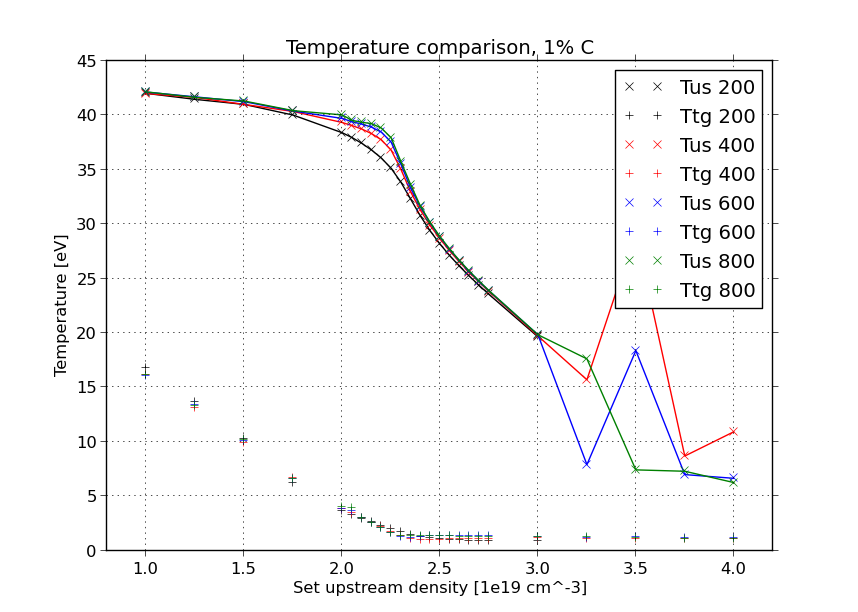
\includegraphics[scale=0.5]{Figures/sol1d/TT_IMPCOMBO2.png}
\centering
\caption{Comparison of $T_{upstream}$ and $T_{target}$ at varying set $n_{e~upstream}$ for different y-axis resolutions in SOL1D}\label{figTT_IMPCOMBO2}
\end{figure}

Simulations from \noNe{3} onwards shown in figure~\ref{figTT_IMPCOMBO2} are detaching and reattaching in quick succession, so they are unlikely to approach a steady state within a reasonable number of timesteps. When detached, the upstream temperatures in these simulations follow the downward trend observed with increasing \neus. However, when the system destabilises and rushes to reattach to the target plates, the upstream temperature shoots up. If these higher density simulations are terminated during a period of detachment, \Tus will be low, as is the case for all the \noNe{3.75} runs. Conversely, if they are terminated when the density profile has reattached, \Tus will be much higher, which can be seen in the data points at \noNe{3.5} for ny = 400 \& 600 cells. 

This cyclical detachment and reattachment is portrayed in figure~\ref{figny400800r35netg} - here sheath density, \netg, is observed following a pattern of peaks (when system is attached to the target) and troughs (when the system is detached). In the case of the black line, with y-axis resolution of 400 cells, the simulation has stopped when the sheath density is still far higher than its minimum value, so the density profile is still in the process of detaching from the target surface. Consequently, the upstream temperature is still relatively quite high. The red line is from a simulation with the same input values but using 800 cells along the y-axis, here termination has occurred when the density profile is almost fully detached from the target, hence the upstream temperature is quite low. This termination snapshot effect can be seen in figure~\ref{figTT_IMPCOMBO2} at \noNe{3.5}, where the upstream temperature with 400 cells is much higher than that for 800 cells.

\begin{figure}
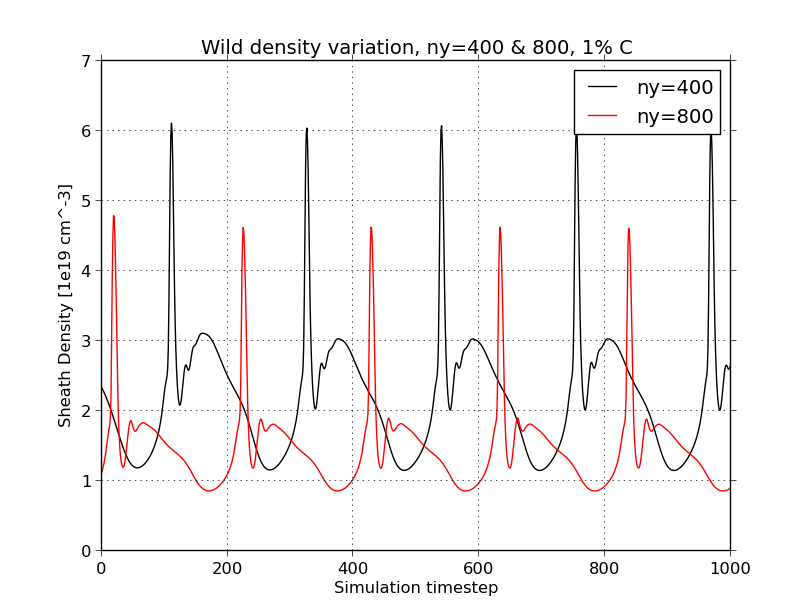
\includegraphics[scale=0.5]{Figures/sol1d/ny400800r35netg.png}
\centering
\caption{Continual detachment and reattachment causes the target $n_e$ variations for ny = 400 and 800 cells run with \neus~set to \noNe{3.5}.}\label{figny400800r35netg}
\end{figure}

\subsection{Pressure Loss}\label{ssecPloss}
Pressure ratio $2\frac{P_{tg}}{P_{us}}$ was calculated for the density scan data with different resolutions and plotted against target plate temperature in figure~\ref{figPL_IMPCOMBO2logy}; the data from varied resolutions show good agreement. Experimentally, pressure loss ratio saturates to unity at high target temperatures due to the relation between static and dynamic pressure and falls as \Ttg decreases, after the system has started to detach. Experimental pressure loss data from Alcator C-Mod is displayed in figure~\ref{figPlossAlcator}. The sharp drop in pressure loss ratio below 3 eV is thought to be caused by atomic effects which become relevant at those lower temperatures \cite{Pitcher1997}.

Pressure loss saturation is not observed in the simulations shown in figure~\ref{figPL_IMPCOMBO2logy}, and this discrepancy is expected to be due to the way ion viscosity is handled in the model. Ion viscosity varies like $\eta_i \propto \tau_i T \propto T^{\frac{5}{2}}$, where $\tau_i$ is the ion collision time, hence this term in the overall viscosity equation is likely to blow up at higher temperatures, which would lead to the lack of saturation seen here. 

\begin{figure}
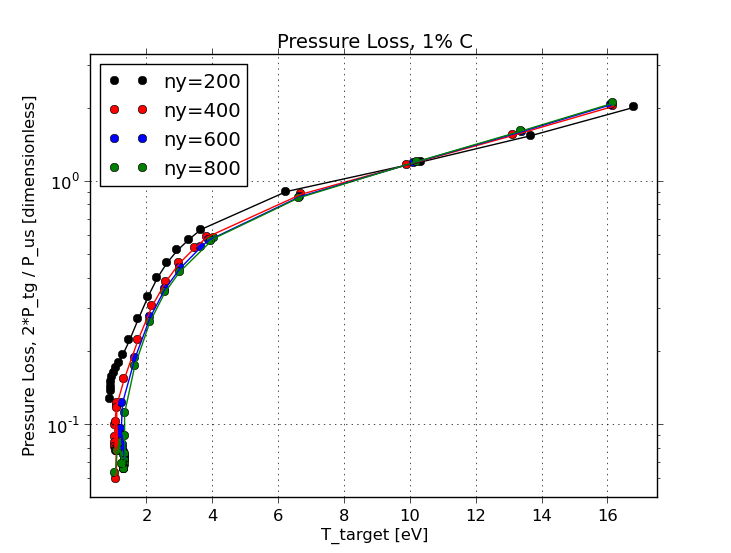
\includegraphics[scale=0.5]{Figures/sol1d/PL_IMPCOMBO2logy.png}
\centering
\caption{Pressure loss ratio, $\frac{2P_{tg}}{P_{us}}$, change with \Ttg at different y-axis resolutions in SOL1D.}\label{figPL_IMPCOMBO2logy}
\end{figure}

\begin{figure}
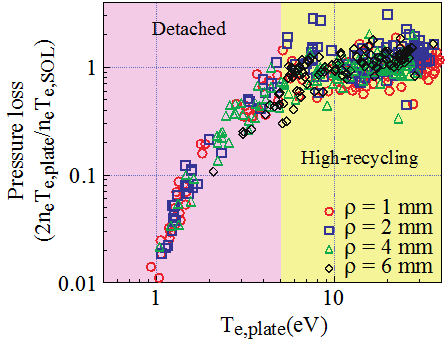
\includegraphics[scale=0.7]{Figures/PlossAlcator.png}
\centering
\caption{Pressure loss ratio, $\frac{2P_{tg}}{P_{us}}$, against divertor plate temperature. Data from Alcator C-Mod \cite{Lipschultz2007}. The $\rho $ values show the distance of the four different radial flux surfaces from the midplane.}\label{figPlossAlcator}
\end{figure}

SOL pressure is a combination of the static thermal pressure and the dynamic pressure, which is due to the motion of the ions. Pressure loss between the upstream and the target is caused by the friction between the plasma and the neutrals. In much of the SOL, the thermal velocity is greater than the ion velocity, so $P_{static}~\gg~P_{dynamic}$. However, at the sheath, ion velocity is equal to the sound speed, making the two pressures equal. As \neus increases, so does pressure loss, because a larger number of particles in the same volume leads to greater friction between the plasma and neutrals.


\subsection{Ion Viscosity}\label{ssecIonviscosity}
To study the lack of saturation at higher \Ttg values, seen in figure~\ref{figPL_IMPCOMBO2logy}, simulations were run ignoring the effects of ion viscosity, $\eta_i$, in the system. As discussed in section~\ref{sssecPloss}, $\eta_i$ varies with $T^{5/2}$, so it is likely to blow up at high temperatures. When removing the effects of ion viscosity, the saturation observed experimentally is seen in the simulation data, which is shown in figure~\ref{figPL_iVpts}. Ignoring ion viscosity results in higher average ion velocity in the target area and hence higher target temperature, which is the drawback to removing these effects from the system. Another drawback is that these simulations take significantly longer to reach near steady-state conditions, as ion viscosity is a large contributor to damping in the system.

A possible method of retaining the pressure loss saturation alongside viscous ion properties would be to introduce a flux limiter into the SOL1D framework. The current heat flux model \cite{Braginskii1965} fails to come close to the real value at high temperature gradients, because it approximates heat flux as varying linearly with $\nabla T$ which misses the asymptote at $q_max$. This limit exists because heat in a system cannot flow faster than the electron thermal velocity.

\begin{figure}
	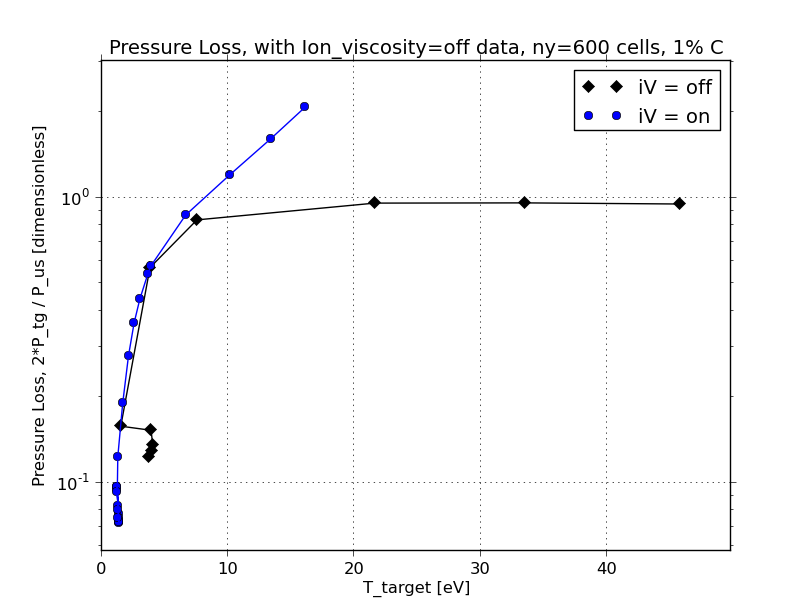
\includegraphics[scale=0.5]{Figures/sol1d/PL_iVpts.png}
	\centering
	\caption{Pressure loss data with and without the effects of ion viscosity, $\eta_i$, the inclusion of which prevents pressure loss saturation at higher \Ttg. This comparison was run in conventional divertor geometry.}\label{figPL_iVpts}
\end{figure}

Free-streaming thermal conductivity provides a better model of plasma heat flow, and is implemented in the 2D version of SOL1D, Hermes-1. To ensure future applicability of SOL1D results, a flux limiter could be implemented in the model to impose the electron thermal speed as the maximum possible heat transfer speed.



\subsection{Radiated Power}\label{ssecRpower}
SOL1D considers three types of radiated power: radiation due to impurities, Rzrad; due to ionisation, Riz and due to recombination, Rrec, which are combined to give total radiated power, R. An interesting quantity calculated from these three sources is the radiated power flux, $ \hat{P}/A $, at a given time point in a simulation. This is given in equation~\ref{eqRpflux}, where $e$ is the charge of an electron, $\omega_{ci}$ is the ion cyclotron frequency and $dy$ is the simulation cell spacing. $\hat{N}$ and $\hat{T}$ are density and temperature normalisation factors, and $ A $ is the cross sectional area of the flux tube. We analysed the data of the blue curve in figure~\ref{figTT_IMPCOMBO2} in this radiation section. 

\begin{equation}\label{eqRpflux}
\hat{P}/A = (R~e~\hat{N}~\hat{T}~\omega_{ci}) \times dy
\end{equation}

\begin{figure}
\transparent{0.75}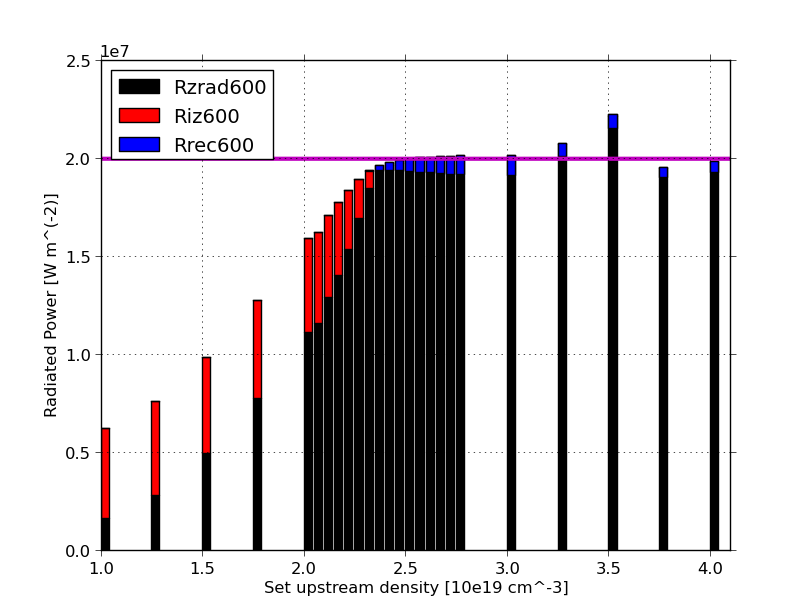
\includegraphics[scale=0.5]{Figures/sol1d/PRbar600.png}
\centering
\transparent{1}\caption{Different sources of radiated power at varying set upstream density in SOL1D, with ny = 600 cells. The horizontal line shows the upstream power flux input.}\label{figPRbar600}
\end{figure}

Radiated power flux as a fraction of power flux input is expected to be lower at smaller values of \neus because system temperature is higher overall, and most plasma species are fully ionised. This is observed in figure~\ref{figPRbar600}, along with more power radiated as \neus increases and the system undergoes detachment, reducing the average temperature, a trend which can be seen in figure~\ref{figTT_IMPCOMBO2}. As the temperature falls, more species begin to recombine, especially the carbon impurities. This is why an increase in radiation due to impurities, Rzrad, is observed up to a density of \noNe{2.5}, because carbon can recombine at higher temperatures than the other plasma species, providing significant power loss via Bremsstrahlung and energy level transitions.

Several of the higher \neus runs in figure~\ref{figPRbar600} show the system radiating more power than it receives. Neutrals formed in SOL1D come off the walls with a certain energy which is then transferred to the plasma. Hence, if enough neutrals transfer their energy to the plasma in one time step, the total power radiated can exceed the power input.


\subsection{Particle Transfer}\label{ssecPtrans}
Neutrals recombining from the target and walls and entering the divertor leg travel into the upstream until they are ionised. The position of the density profile peak is strongly coupled to spatial variation of the neutral sink by ionisation as detachment progresses. This can be seen in figure~\ref{figbalSizthick20m}, where the vertical dashed lines show the electron density profile peak position at different stages of detachment. Neutrals' ionisation mean free paths lengthen as the overall SOL temperature falls because their atomic electrons are less likely to be given sufficient energy to overcome the ionisation barrier.

\begin{figure}
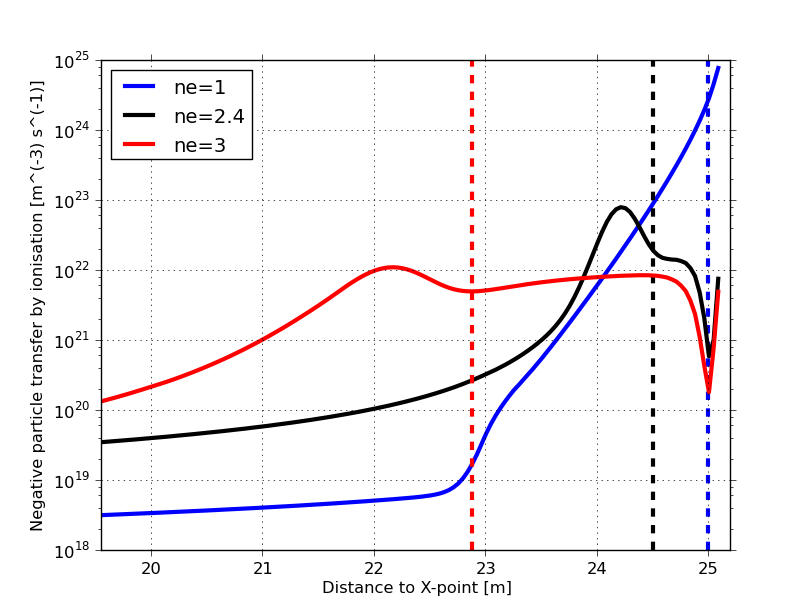
\includegraphics[scale=0.5]{Figures/sol1d/balSizthick20m.png}
\centering
\caption{Spatial distribution of particle transfer through ionisation. All solid lines are negative, which shows neutrals becoming ions, and dashed vertical lines show the position of the corresponding electron density peak.}\label{figbalSizthick20m}
\end{figure}


\subsection{Energy Transfer}\label{ssecEtrans}
Plasma-neutral energy transfer through charge exchange shows some interesting changes as the system detaches from the target plates. Pre-detachment, the plasma loses energy to the neutrals when hot ions pick up electrons from a colder neutrals, producing hot neutrals and cold ions. In the midst of detaching, the ions and neutrals alternate being hottest in distinct regions, from the target plate to 2 metres into the upstream, shown by the black curves in figure~\ref{figbalEcx19m} at \neus = \noNe{2.4}. Electron heat transport is rapid, so they are cooled fastest further away from the plates during detachment. When charge exchange occurs, the ion temperature, $T_i$, is effectively swapped for the neutral temperature, $T_n$. Ions and electrons are strongly coupled in SOL1D, $T_i = T_e$, therefore; the more cool electrons that permeate into the upstream, the more charge exchange reactions will be swapping cold $T_e$ for hotter $T_n$.

\begin{figure}
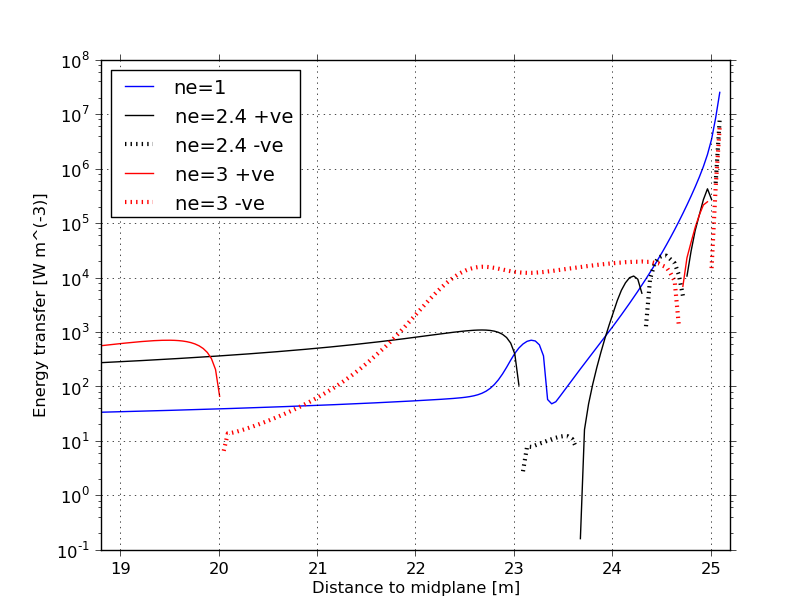
\includegraphics[scale=0.5]{Figures/sol1d/balEcx19m.png}
\centering
\caption{Spatial distribution of energy transfer via charge exchange in CD geometry. Solid lines represent energy being lost to the neutrals by the plasma, while dotted lines show regions where neutrals transfer energy to the plasma.}\label{figbalEcx19m}
\end{figure}


\textbf{MOMENTUM TRANSFER IN CHARGE EXCHANGE THOUGHTS}
Fcx figure: area of negative Fcx (neutrals transfering momentum to plasma) moves toward upstream as detachment progresses. Perhaps fast neutrons making it past the detachment peak (as their interaction cross section is lower due to their higher velocity) then make it to a region where they have greater speed than the ions in that region (which are being continually accelerated from the moment they enter the upstream at v=0) and therefore transfer momentum TO the ions in that region. Lab book sketch depicts what happens. This reduces the hot ion flux to the target and allows the area close to the plates detach and cool further.



\subsection{Super-X Geometry}\label{ssecSXG}
Until now, the SOL1D simulations performed have used a standard divertor geometry and parameters (25m long field line and uniform B-field). Future simulations aim to emulate behaviour of MAST-Upgrade, which has just installed a Super-X divertor (SXD) in place of it's previous conventional divertor (CD); the differences between the two can be seen in figure~\ref{figCDvsSXD}. In the SXD geometry, the distance from the X-point to the target is much longer than the CD set up. Additionally, extra magnetic coils have been added into the nose of the bulkhead seen extending towards the X-point, which further separate the cold divertor plasma from the bulk plasma. These factors allow a greater tolerance when implementing conditions to achieve detachment, as changes in the divertor region are not transmitted as quickly or with the same magnitude as with the CD geometry.

\begin{figure}
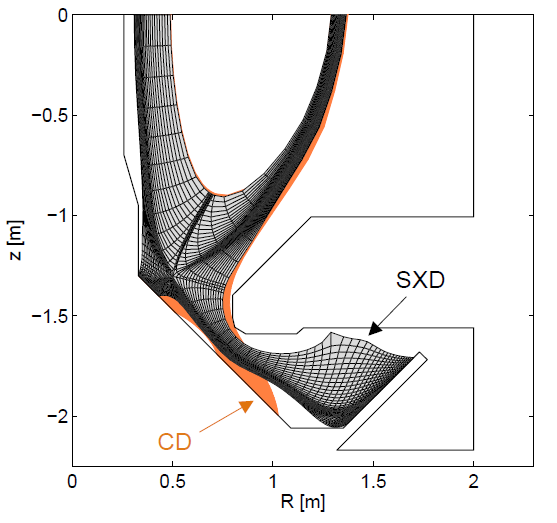
\includegraphics[scale=0.5]{Figures/CDvsSXD.png}
\centering
\caption{A comparison of the Super-X Divertor (SXD) and the Conventional Divertor (CD) geometries on MAST \cite{Havlickova2014}. The y-axis, z, is the height in metres and R is the major radius, in metres.}\label{figCDvsSXD}
\end{figure}

Implementing this new geometry requires estimating how the magnetic field changes over the length of the field line. This is entered into the simulations by changing the Area Expansion Ratio (AER), which describes how the cross section of a flux tube changes as it traverses the length of the field line. A distance of $0.005$ m out from the separatrix into the SOL was used, thus by using the third panel in figure~\ref{figMASTUdesignpapersFig2} the AER is estimated to be 12. Furthermore, the connection length of the field line between the X-point and the target is estimated as $26$ m, from the second panel in figure~\ref{figMASTUdesignpapersFig2}. The connection length between the outboard midplane and the X-point is $5$ m \cite{Fishpool2013}, making the total length of the simulation y-axis $31$ m. The fourth panel in figure~\ref{figMASTUdesignpapersFig2} shows the distribution of connection length, for a field line 0.01 m into the separatrix, between the midplane and the target plates \cite{Fishpool2013}. The first pane in figure~\ref{figMASTUdesignpapersFig2} shows the divertor leg footprints for each configuration.

\begin{figure}
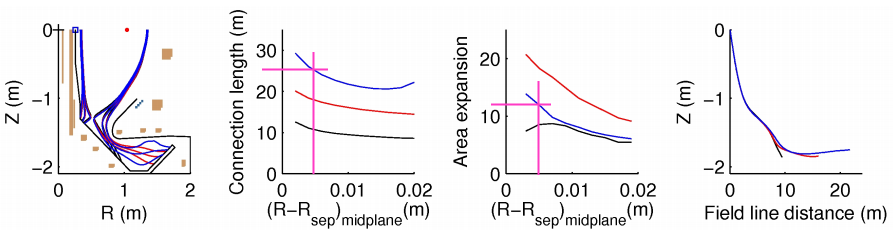
\includegraphics[scale=0.75]{Figures/MASTUdesignpapersFig2_2.png}
\centering
\caption{Representative magnetic equilibria with full toroidal field (0.8T vacuum at R=0.8m) showing conventional (black), expanded strike point (red) and Super-X like long connection length (blue) divertor geometries on MAST \cite{Fishpool2013}. Z is height, R is major radius, $ R_{sep} $ is the radius from the machine centre to a point in the separatrix, so $ R - R_{sep} $ is a distance from the plasma edge into the separatrix. The pink lines on panels 2 and 3 highlight our choice of connection length and area expansion for the SXD geometry.}\label{figMASTUdesignpapersFig2}
\end{figure}

The extended divertor leg in the SXD geometry enables simulations to settle down far quicker than in the CD set up, as the power input (at the midplane) is much farther removed from the complicated and delicately balanced interactions at the target.


\subsection{Neutral Loss}\label{ssecNloss}
Rate of neutral loss, $nloss$, in the divertor leg can vary largely depending on their interaction mean free path, $\lambda_{mfp}$. If $\lambda_{mfp}$ becomes comparable to the width of the plasma channel in the leg then neutral lifetime in the plasma will become very short. We set neutral loss rate to $1\e{3}$ s\pow{-1} for all previous simulations. Increasing \neus initially increases $j_{sat~tg}$, as the ion flux to the target is higher. However, once detachment begins, ion density near the target starts to fall as the plasma density profile shifts away from the divertor plate. This leads to the roll-over region in the $j_{sat~tg}$ profile, as $j_{sat~tg} \approx nv_{i~tg}$, the plasma flux at the target.

Using the super-X geometry, $nloss$ was varied between 1\e{3} and 1\e{5} s\pow{-1}. Saturation current density at the sheath, $j_{sat~tg}$, was plotted against upstream density at various values to provide the $j_{sat~tg}$ profiles shown in figure~\ref{fignloss1e345,52.5e425_2}. Increasing $nloss$ has a stark effect on the roll over region of the $j_{sat~tg}$ profile, it moves to higher density as $nloss$ increases. The initial $j_{sat~tg}$ gradient changes significantly with $nloss$. At loss rate $1\e{4}$ s\pow{-1} the gradient grows initially, then decreases when detachment starts and $j_{sat~tg}$ begins to fall. In contrast, the $j_{sat~tg}$ profile gradients for the higher $nloss$ runs are always decreasing even at low \neus. 

\begin{figure}
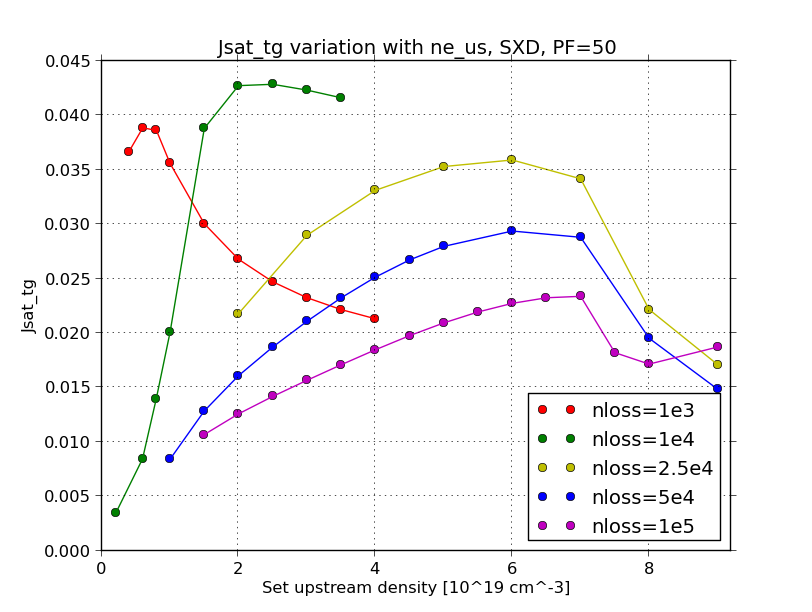
\includegraphics[scale=0.5]{Figures/sol1d/nloss1e345,525e425_2.png}
\centering
\caption{Saturation current density at the sheath, $j_{sat~tg}$ vs. upstream density, \neus, at different neutral lifetimes, nloss. Nloss has units of [s\pow{-1}]. SXD geometry was used for all simulations here.}\label{fignloss1e345,52.5e425_2}
\end{figure}

Several lower density simulations failed at all values of $nloss$, which is likely due to particles leaving the system too quickly for the density controller in the upstream to adjust. Once a lot of particles leave the system, because the power input stays the same, the overall temperature increases. Ion velocity into the sheath is set to the sound speed, and $v_S \propto \sqrt{T}$, so the rate of particles leaving the system into the sheath increases. This produces a vicious cycle as the temperature keeps increasing while more particles leave the system, and particles leave the plasma faster the higher the temperature. Further work could be done to try to stabilise the failed low density, high $nloss$ simulations in order to better understand the relationship between neutral loss rate and $j_{sat~tg}$ in the ramp up phase.



\subsection{Impurity Fraction}\label{ssecImpfrac}
Impurity fraction in the divertor heavily influences the amount of power lost to radiation, as impurities are a largest contributor to volumetric radiative power loss in a hydrogenic plasma. SOL1D takes an input that sets the percentage of carbon impurity in the system. Figure~\ref{figCvarPL5nes} shows the pressure loss ratio at different impurity fractions and upstream densities against the target temperature. Interestingly, all the profiles follow the same overall curve, which suggests that pressure loss is a function of the energy loss, because increasing the impurity fraction does not add any more friction to the system. Therefore, the additional loss of pressure as the percentage of carbon goes up is due to the extra energy loss from impurity radiation.

\begin{figure}
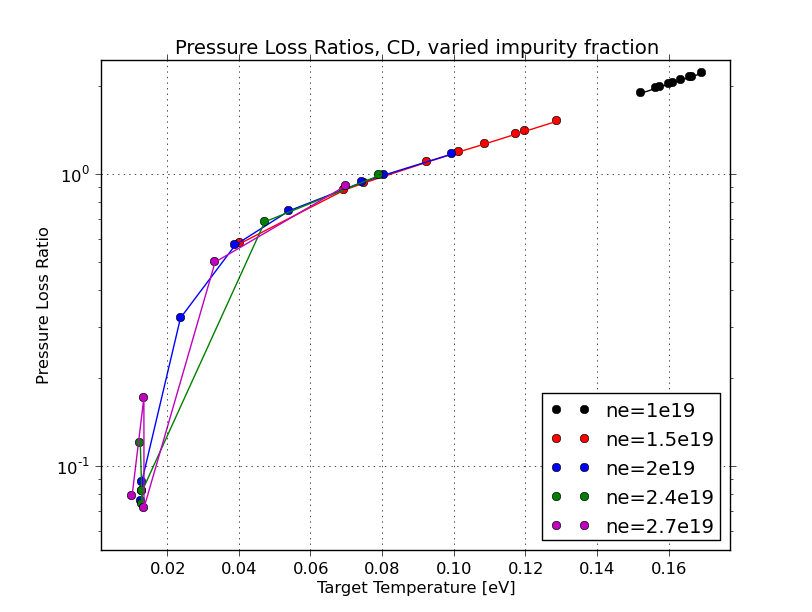
\includegraphics[scale=0.5]{Figures/sol1d/CvarPL5nes.png}
\centering
\caption{Pressure loss ratio, $2P_{tg}/P_{us}$ vs target temperature, \Ttg, in CD geometry. Impurity fraction was changed to give the five different curves are at varied \neus. Densities 1, 1.5 and \noNe{2} were run with impurity percentages 0, 0.4, 0.5, 0.8, 1.0, 1.2, 1.5, 1.6 and 2.0. Whereas densities 2.4 and \noNe{2.7} were run with 0, 0.5, 1.0, 1.5 and 2.0.}\label{figCvarPL5nes}
\end{figure}

Examining the spread of values at each \neus in figure~\ref{figCvarPL5nes}, impurity fraction has an increasing affect on the pressure loss as \neus increases. At the lowest upstream density the effect of increasing the carbon fraction does not lead to any significant change in the progress of detachment. Following a 50\% density increase to \noNe{1.5}, the carbon fraction change causes a fivefold wider \Ttg spread, and this range is at least as wide again for \noNe{2}. A higher \neus at fixed power input leads to a lower overall temperature, which in turn leads to more radiative energy loss as more ions, hydrogenic and carbon, recombine with electrons which then transition to lower atomic electron levels, radiating away more energy. Carbon in the plasma itself does not introduce extra friction to cause the observed loss of pressure, however; as the average temperature falls, friction between the plasma and neutrals will increase. This is because neutral penetration will extend further into the upstream as temperature drops, detailed in section~\ref{ssecPtrans}, due to the fact that their ionisation mean free path is longer.

Near 4 eV in figure~\ref{figCvarPL5nes} lie points from the red, blue and purple sets, showing that system state over large density gaps can be bridged simply by varying impurity fraction. Here, the blue (\neus = \noNe{2}) point has 1\% impurity concentration, which is the same data as the blue point at the same density in figure~\ref{figTT_IMPCOMBO2}, and is at the beginning of detachment. Hence the overlapping point from the \noNe{1.5} set, 2\% carbon, has been brought to the cusp of detachment, compared to the same density in figure~\ref{figTT_IMPCOMBO2}, by doubling the impurity fraction. The purple point here is at 0.5\% carbon, highlighting that just half a percent lower impurity concentration in a plasma can bring it from complete detachment (see \neus = \noNe{2.7} points in figure~\ref{figTT_IMPCOMBO2}) to a position where detachment is only just beginning.

\begin{figure}
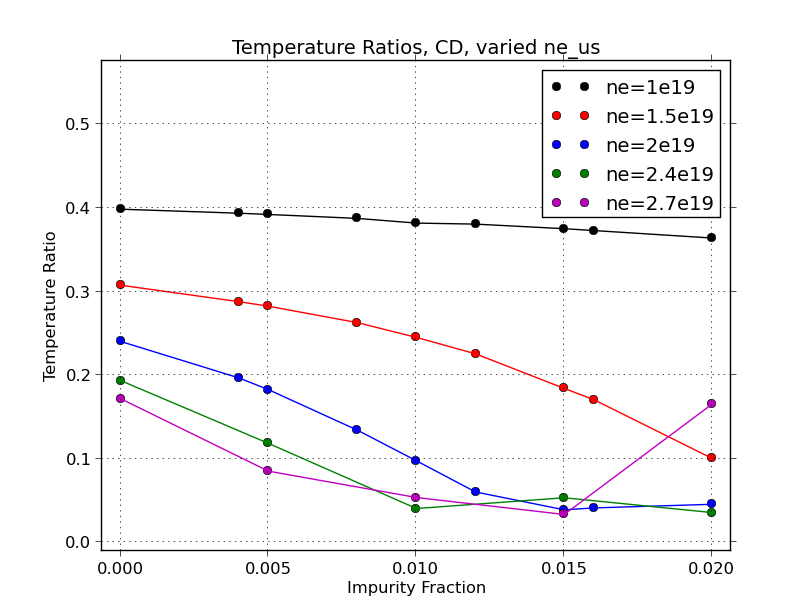
\includegraphics[scale=0.5]{Figures/sol1d/CvarTR5nes.png}
\centering
\caption{Target and upstream temperature ratio against impurity fraction for different upstream densities, in CD geometry.}\label{figCvarTR5nes}
\end{figure}

\begin{figure}
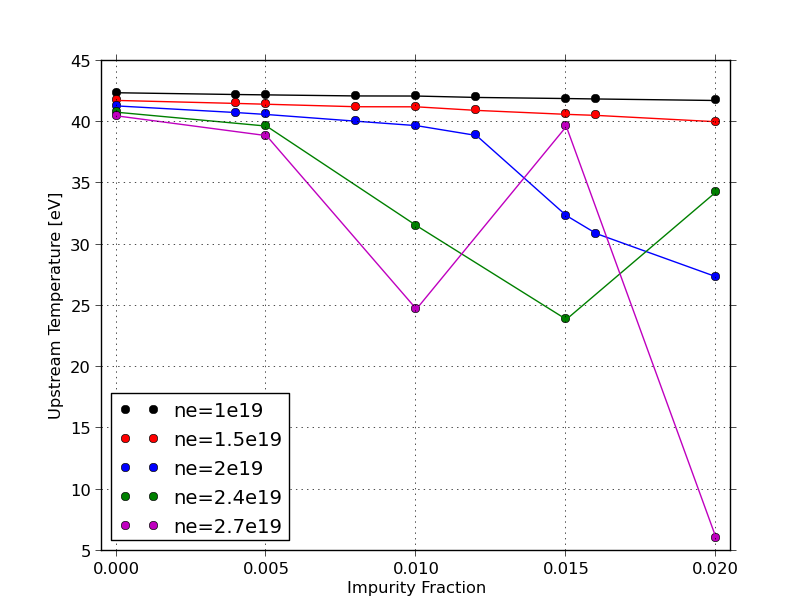
\includegraphics[scale=0.5]{Figures/sol1d/CvarTus.png}
\centering
\caption{Upstream temperature, \Tus, against impurity fraction for different upstream densities, in CD geometry.}\label{figCvarTus}
\end{figure}

Figure~\ref{figCvarTR5nes} shows the temperature ratio, \Ttg/\Tus, and is supported by figure~\ref{figCvarTus}, allowing changes in temperature ratio to be more easily understood. Maintaining a target temperature below 5 eV over a whole shot cycle in a tokamak will require careful control of several parameters which influence the SOL temperature profile. Reducing \Ttg quickly affects \Tus, which directly influences core plasma temperature and fusion performance. An approximate guide for minimum acceptable \Tus is estimated as 90\% of the \neus = \noNe{1} run with 0\% impurities, the first black point in figure~\ref{figCvarTus}, which is 38.2 eV. 

Higher upstream densities require lower impurity levels to bring \Ttg below the required temperature. Successful operation can be achieved at the different densities as follows. At the lowest density examined here, \noNe{1}, carbon percentage will need to be increased further, above 2\%, beyond the scope of this group of simulations. The danger in doing this is the transport of impurities into the core, which can lead to catastrophic Bremsstrahlung energy losses if uncontrolled. For \noNe{1.5}, an accelerating \Ttg decrease, falling threefold over the impurity fraction range, is accompanied by little reduction of \Tus. The window of acceptable carbon percentage shrinks as \neus increases, figure~\ref{figPRbar600} shows that power radiated by impurities quickly swamps all other loss terms as density is increased.

We focused on one set of the impurity fraction data, that at \neus = \noNe{2}.  Figures~\ref{figCvarTRne2} and \ref{figCvarPMne2} show the \Tus and \Ttg data for this case and the density profile peak position respectively. From pure hydrogenic plasma to 1.2\% impurity fraction, as the power radiated by impurities increases the target temperature falls steadily and drops below the 5 eV threshold for long term operation. The window from about 0.85\% to 1.2\% produces the desired \Ttg while retaining a sufficiently high \Tus so as not to hinder core plasma performance significantly. Within this window however, the density profile peak has remained attached to the divertor plate, as figure~\ref{figCvarPMne2} shows. Perhaps a divertor set up could be devised with a carefully controlled impurity population such that it can be held in a \textit{just} attached scenario. In this case the impurity fraction would radiate sufficient power to give an acceptable \Ttg, and progress of the detachment peak need not be closely controlled, as is the worry for the success of detachment in many machines, simply because the plasma in the divertor remains attached. However, after modelling and experimentally measuring impurity transport in the divertor region, strictly controlling the impurity population there may be an unrealistic goal. It has been shown that detachment reduces the compression of impurities in the divertor region \cite{Bosch2001}, so impurity transport during detachment does require further analysis.

Sudden detaching at impurity concentrations above 1.2\% cause a rapid drop in \Tus to such levels as could hinder core temperature. More study should be focused on this small region to better visualise and understand the effect on density peak position and upstream temperature as the plasma detaches from the plate. For ITER's operation, divertor impurity seeding will be necessary to reduce divertor heat fluxes by facilitating detachment \cite{Kallenbach2013}.

\begin{figure}
	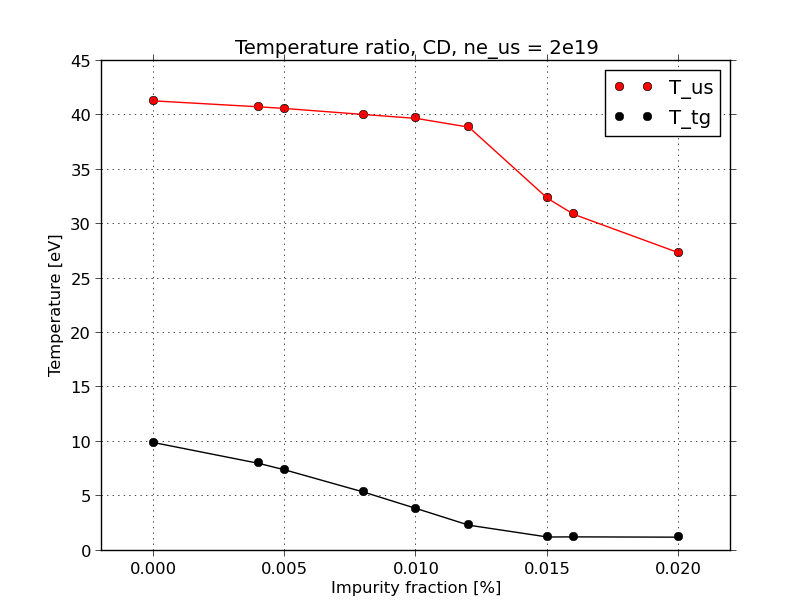
\includegraphics[scale=0.5]{Figures/sol1d/CvarTRne2.png}
	\centering
	\caption{Target and upstream temperature against impurity fraction, at \neus = \noNe{2} in CD geometry.}\label{figCvarTRne2}
\end{figure}

\begin{figure}
	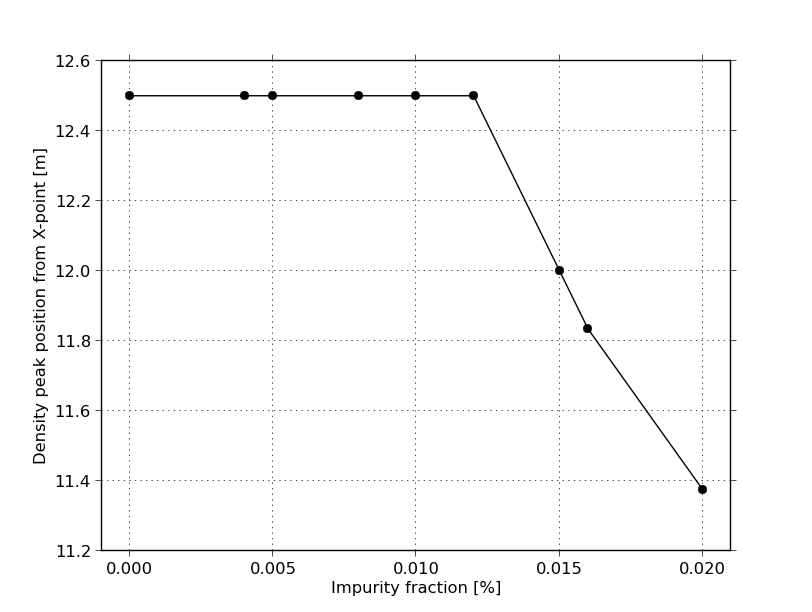
\includegraphics[scale=0.5]{Figures/sol1d/CvarPMne2.png}
	\centering
	\caption{Distance of density peak to the X-point in metres at different impurity fractions, \neus = \noNe{2} in CD geometry.}\label{figCvarPMne2}
\end{figure}



\section{Conclusion}\label{secConclusion}
Power production in fusion power plants after ITER, DEMO and beyond, will most likely increase \cite{Federici2014}, and with that the power entering the SOL will continue to increase. Consequently, the only option to ensure the viability of current divertor designs in these machines, is to develop a concrete understanding of the physics behind detachment. Only then can its stability be ensured and fusion power can begin to challenge current energy production methods. Analysis of the processes causing detachment was made, such as the spatial distribution of plasma particle sinks, and energy and momentum transfer in charge exchange reactions near the divertor plate. The effects of upstream density and impurity fraction on detachment were highlighted, in particular how operating in a controlled range of these parameters could allow the position of the detachment front to be strictly controlled, while retaining a sufficiently cold target for prolonged operation. Further research should be conducted into these operating windows, first using 2D simulations to include cross field transport and to consider detachment at both the inner and outer divertor plates. Following this, 3D simulations should be conducted to assess the effects of turbulence and toroidal asymmetries, before translating the findings into experimental design, where the windows of operation can be more rigorously tested.


\printbibliography

\end{document}
